\begin{frame}
	\frametitle{Aktuelle Nachrichten}
		\begin{figure}
		\centering
		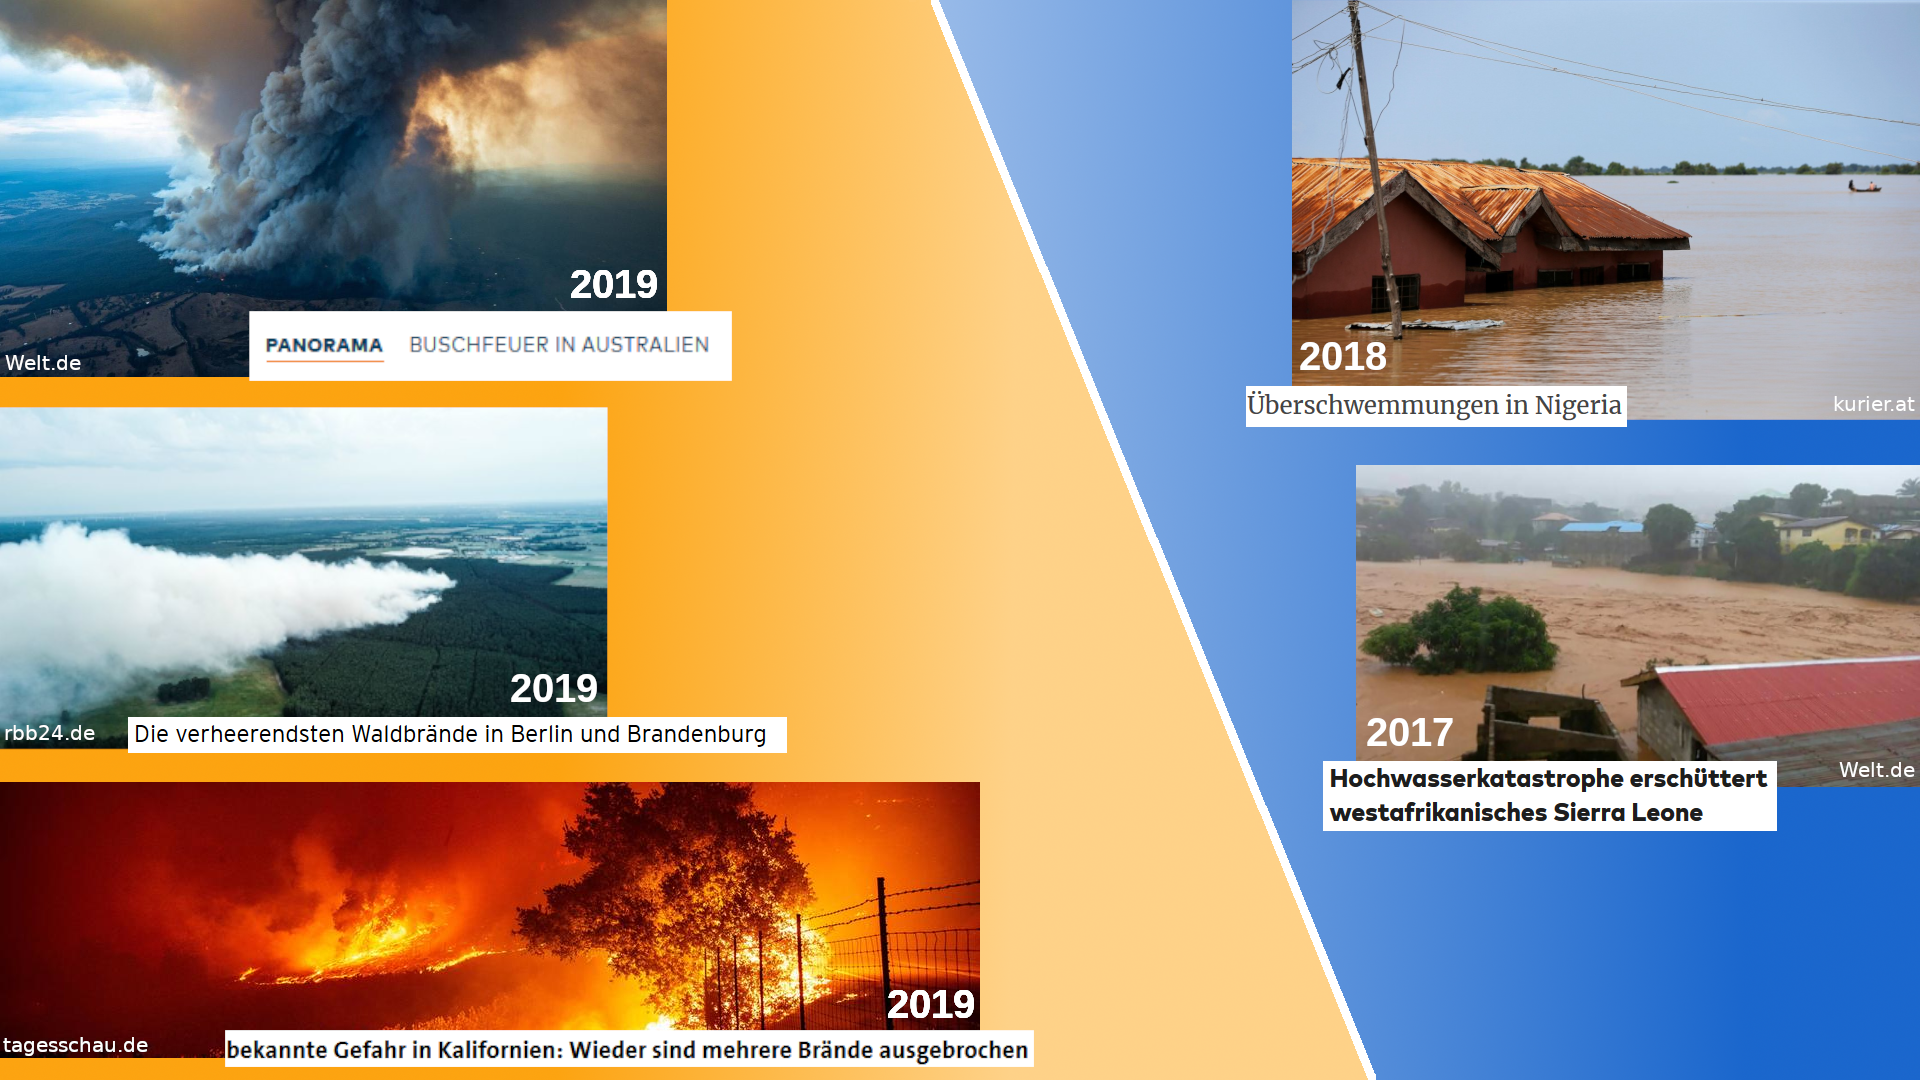
\includegraphics[width=0.9\linewidth]{bilder/CurrentSituation}
		\end{figure}

		\note{
			Wetterereignisse der letzten drei Jahre
			\begin{itemize}
				\item[2017] Hochwasserkatastrophe in Sierra Leone durch bis du dreifach höheren Regenfall als üblich, keine Unwetterwarnung der Regierung, unkontrollierte Entwaldung, Müllverstopfte Kanalisation, etc.
				\item[2018] Überschwemmungen in Nigeria und vielen anderen afrikanischen Ländern, mehrere Millionen Menschen obdachlos
				\item[2019] Buschbrände in Kalifornien, mehr als \SI{1000}{km\squared} (etwa drei mal die Fläche von Dortmund) verbrannt, gehört zu den größten 5 Buschbränden. 4 der größten 5 Brände waren in den letzten 10 Jahren
				\item[2019] Waldbrände in Brandenburg, größte Waldbrände der Geschichte des Landes (etwa 1,5 mal größer als bisher größter),
				etwa \SI{7,50}{km\squared} (etwa die Fläche von Dorstfeld) verbrannt.
				\item[2019] Buschfeuer in Australien, \SI{186000}{km\squared} (\SI{20}{\%} der bewaldeten Fläche Australiens, bzw. \nicefrac{1}{2} mal die Fläche von Deutschland) verbrannt, etwa 1 Mrd. Tiere getötet, Rauch auch in Argentinien und Chile spührbar, wird Black Summer genannt.
				\item[2020] zu warmer und trockener Sommer in Deutschland \SI{1,9}{\celsius} über dem Mittel der Referenzperiode 1961 bis 1990, Waldbrände und Hurrikans in den USA, etc.
				\item[$\rightarrow$] Beobachtung extremer Wetterereignisse
			\end{itemize}
		}
	\end{frame}

\begin{frame}
	\frametitle{Aktuelle Nachrichten}
	\begin{figure}
		\centering
		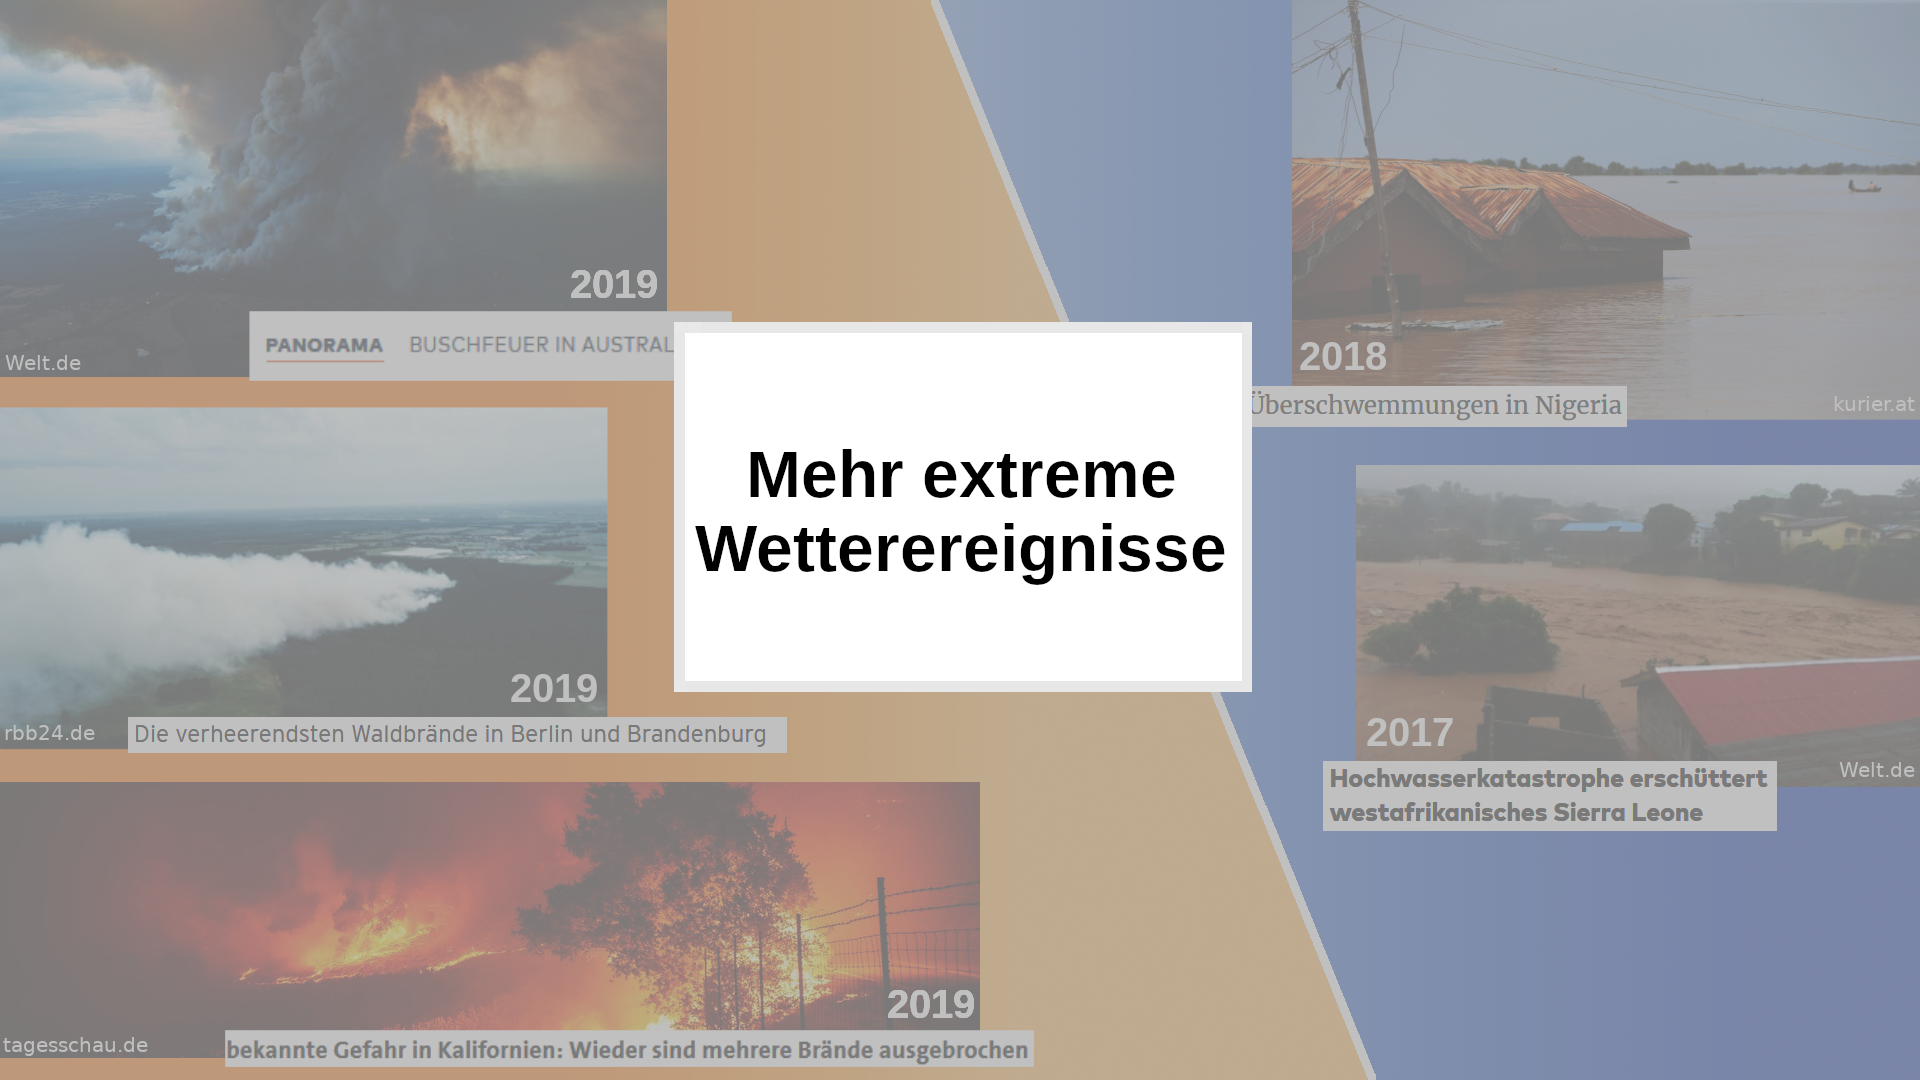
\includegraphics[width=0.9\linewidth]{bilder/CurrentSituation_Conclusion}
	\end{figure}
\end{frame}

\begin{frame}
	\frametitle{Aktuelle Nachrichten}
	\begin{figure}
		\centering
		\begin{tikzpicture}
			\node[anchor=south west,inner sep=0] (image) at (0,0) {
				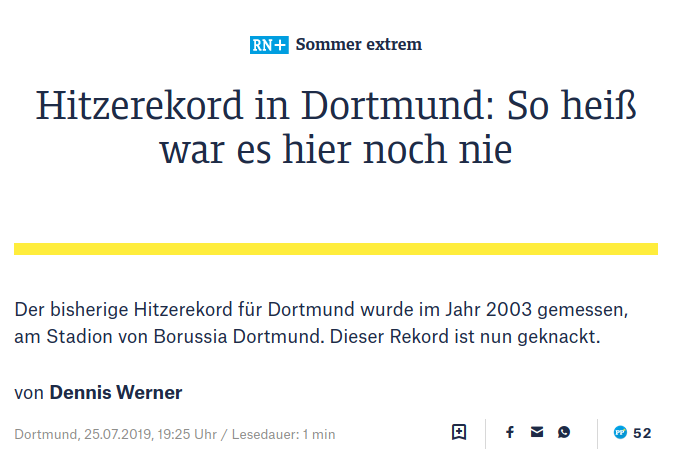
\includegraphics[width=0.7\linewidth]{bilder/dortmund}};
			\begin{scope}[x={(image.south east)},y={(image.north west)}]
				\draw[red,ultra thick,rounded corners] (0.12,0.0475) rectangle (0.23,0.1);
			\end{scope}
		\end{tikzpicture}
	\end{figure}
	\begin{center}
		\textbf{Auch bei uns}
	\end{center}
	\note{
	\begin{itemize}
		\item Man muss gar nicht so weit gehen, in Dortmund ist es genau so (2019)
		\item Extrem Ereignisse lassen sich nicht ausschließlich auf den Klimawandel zurück führen
		\item Statistische Modelle ermöglichen es aber heute zu zeigen, dass Extremereignisse durch den Klimawandel mit einer viel höheren Wahrscheinlichkeit auftreten.
	\end{itemize}
	\vspace{1em}
	Wie sieht das nun global tatsächlich aus?
	}
\end{frame}

% "es war doch immer schon im Sommer warm"


\begin{frame}[t]
	\frametitle{Warming Stripes}
	% Abbildung der Warming Stripes: Die Entwicklung ist wirklich dramatisch

	% Farbskala erklären
	\begin{figure}
		\centering
		\vspace{-1em}
		\begin{tikzpicture}
			\node[anchor=south west,inner sep=0] (image) at (0,0) {
			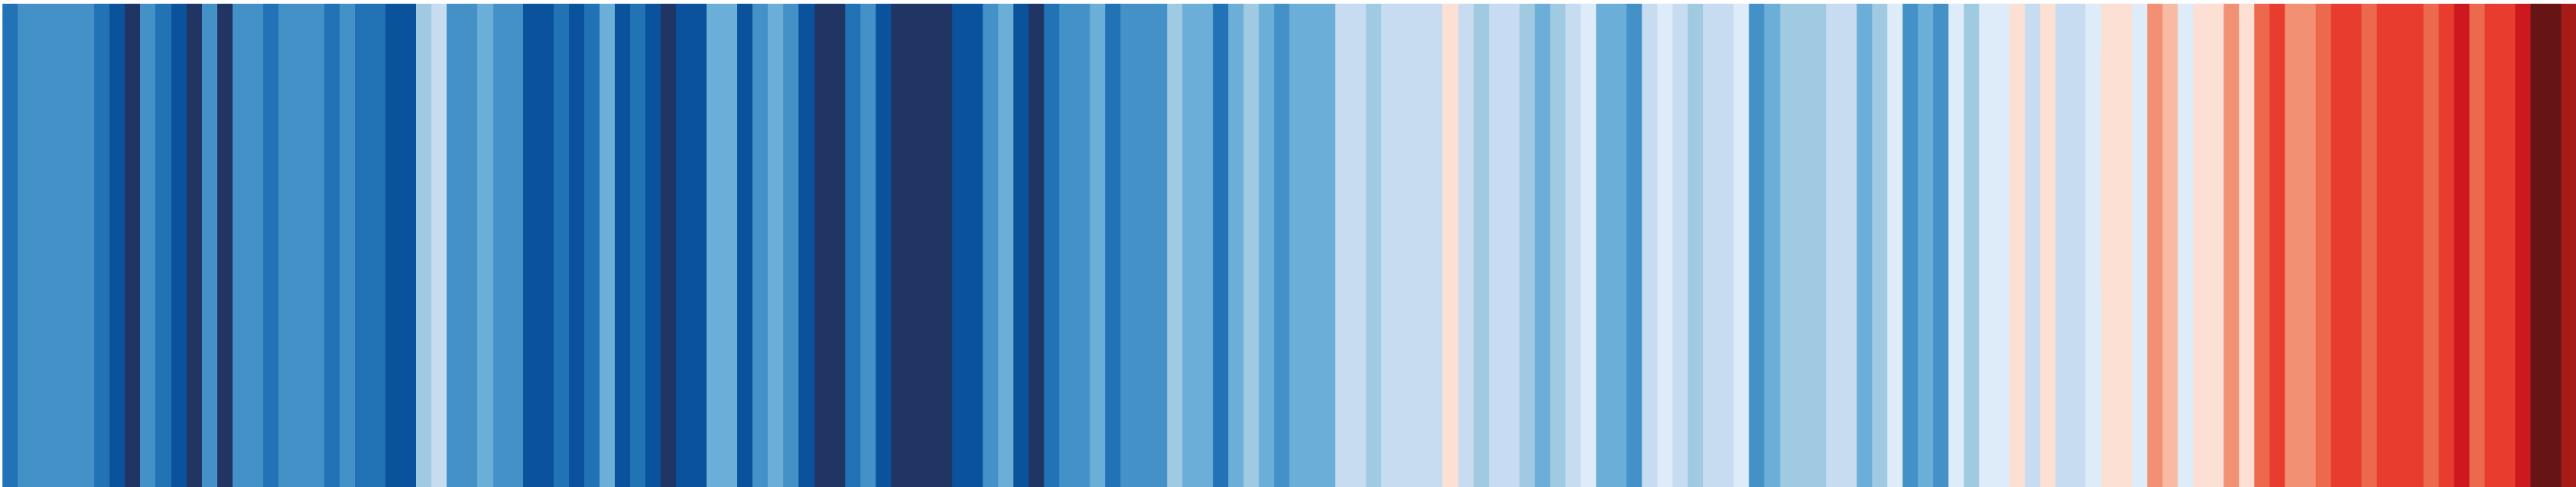
\includegraphics[width=\linewidth]{bilder/s4f-warming-stripes}};
			\begin{scope}[x={(image.south east)},y={(image.north west)}]
				\only<1|handout:1>{\draw[thick,->] (0.0, -0.1) -- (1.0, -0.1) node[anchor=north west] {Zeit};}
				% +/- 0.0058 shifts by one year
				\only<2|handout:0>\fill[gray, opacity=0.7] (0.00,0.003) rectangle (0.3875+0.0058,0.99);
				\only<2|handout:0>\fill[gray, opacity=0.7] (0.3933+0.0058,0.003) rectangle (1.00,0.99);
				\only<3|handout:0>\fill[gray, opacity=0.7] (0.00,0.003) rectangle (0.3875-25*0.0058+0.0025,0.99);
				\only<3|handout:0>\fill[gray, opacity=0.7] (0.3933+5*0.0058+0.0005,0.003) rectangle (1.00,0.99);
				\only<4|handout:0>\fill[gray, opacity=0.7] (0.00,0.003) rectangle (0.3875+5*0.0058+0.0065,0.99);
				\only<4|handout:0>\fill[gray, opacity=0.7] (0.3933+36*0.0058-0.0003,0.003) rectangle (1.00,0.99);
				\only<5|handout:0>\fill[gray, opacity=0.7] (0.00,0.003) rectangle (0.3875+37*0.0058-0.0003,0.99);
				\only<5|handout:0>\fill[gray, opacity=0.7] (0.3933+67*0.0058-0.002,0.003) rectangle (1.00,0.99);
				\only<6|handout:2>\fill[gray, opacity=0.7] (0.00,0.003) rectangle (0.3875+68*0.0058-0.002,0.99);
				\only<6|handout:2>\fill[gray, opacity=0.7] (0.3933+98*0.0058-0.0035,0.003) rectangle (1.00,0.99);
				\only<7|handout:0>{\draw[thick,->] (0.0, -0.1) -- (1.0, -0.1) node[anchor=north west] {Zeit};}
			\end{scope}
	\end{tikzpicture}
		\caption{Die \textit{Warming Stripes}}
		\label{fig:s4f-warming-stripes}
	\end{figure}
	\only<1|handout:1>{
	\begin{itemize}
		\item Jeder Balken repräsentiert eine Jahr aus der Periode 1850-2017
		\item Blau = kälter als der Mittelwert, Rot=Wärmer
		\item Je dunkeler die Farbe, desto extremer die Abweichung vom Mittelwert
		\item Die Trend geht klar zu höheren Temperaturen
		\item Übrigens auch das Logo der Scientists 4 Future
	\end{itemize}
	\begin{center}
		\url{https://s4f-dortmund.github.io/}
	\end{center}
	}
	\only<3|handout:0>{
		\begin{figure}
			\centering
			\vspace{-1em}
			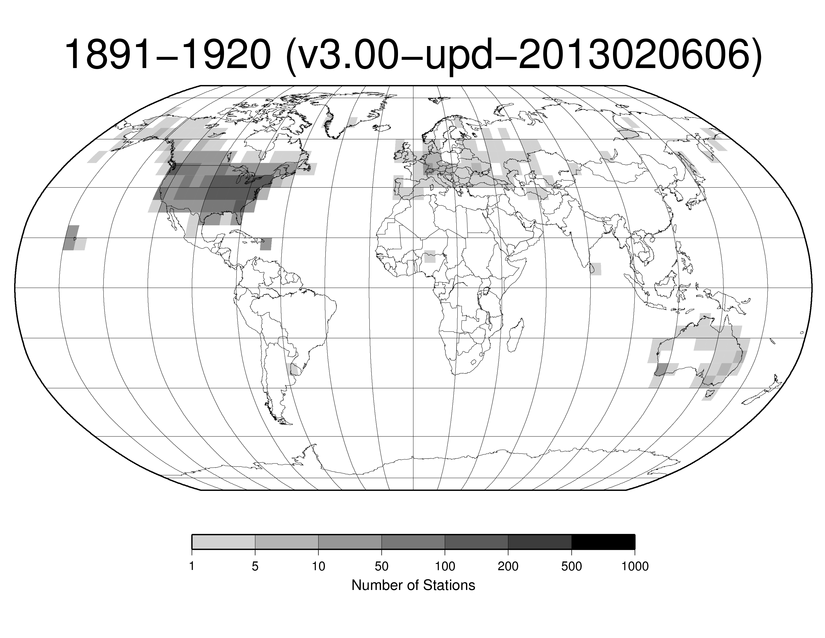
\includegraphics[trim={0cm 1.5cm 0cm 3cm}, clip, width=.425\textwidth]{bilder/Global_Historical_Climate_Network_Daily/station-counts-1891-1920-temp.png}
			\vspace{-1em}
			\caption{Wetterstationen in der Periode 1891 - 1920 die zehn Jahre lang
							 Wetterdaten übertragen haben, Quelle: Global Historical Climate Network}
		\end{figure}
	}
	\only<4|handout:0>{
		\begin{figure}
			\centering
			\vspace{-1em}
			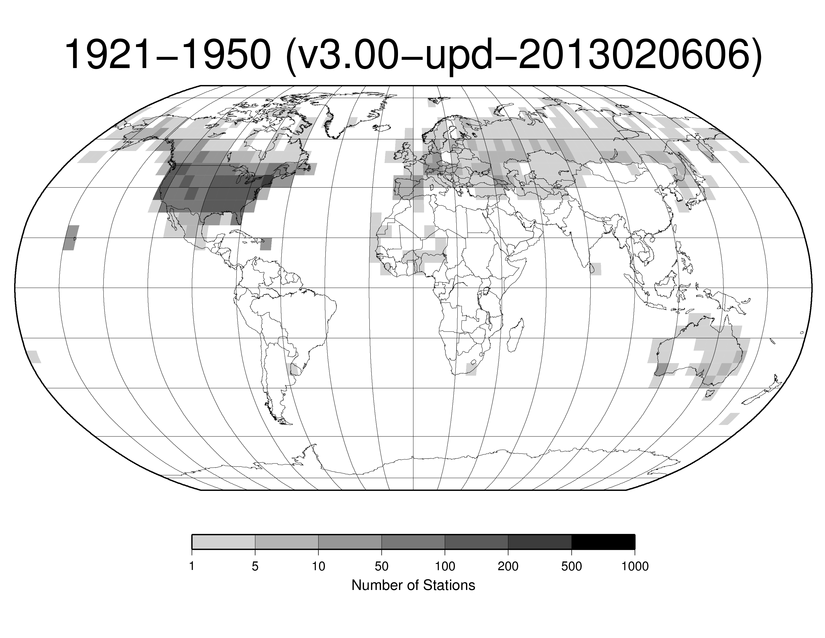
\includegraphics[trim={0cm 1.5cm 0cm 3cm}, clip, width=.425\textwidth]{bilder/Global_Historical_Climate_Network_Daily/station-counts-1921-1950-temp.png}
			\vspace{-1em}
			\caption{Wetterstationen in der Periode 1921 - 1950 die zehn Jahre lang
							 Wetterdaten übertragen haben, Quelle: Global Historical Climate Network}
		\end{figure}
	}
	\only<5|handout:0>{
		\begin{figure}
			\centering
			\vspace{-1em}
			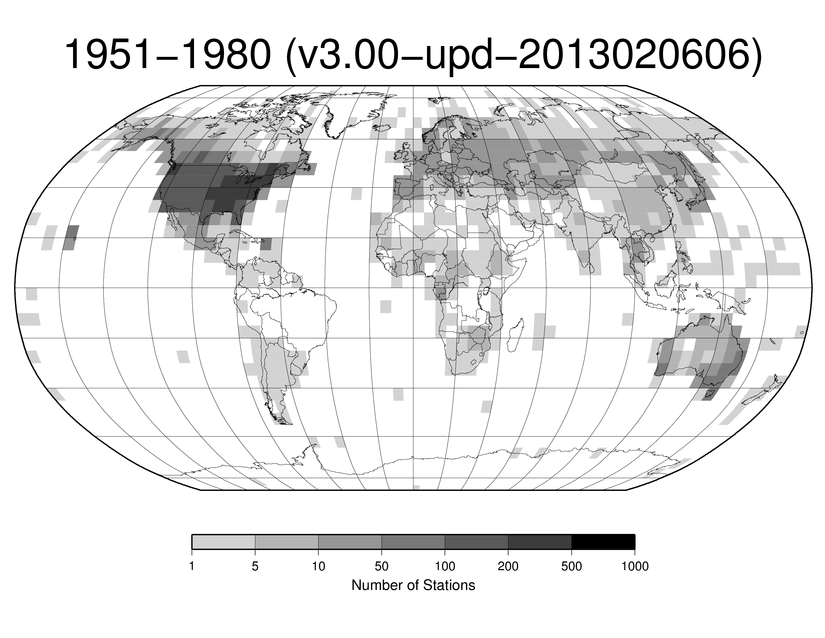
\includegraphics[trim={0cm 1.5cm 0cm 3cm}, clip, width=.425\textwidth]{bilder/Global_Historical_Climate_Network_Daily/station-counts-1951-1980-temp.png}
			\vspace{-1em}
			\caption{Wetterstationen in der Periode 1951 - 1980 die zehn Jahre lang
							 Wetterdaten übertragen haben, Quelle: Global Historical Climate Network}
		\end{figure}
	}
	\only<6|handout:2>{
		\begin{figure}
			\centering
			\vspace{-1em}
			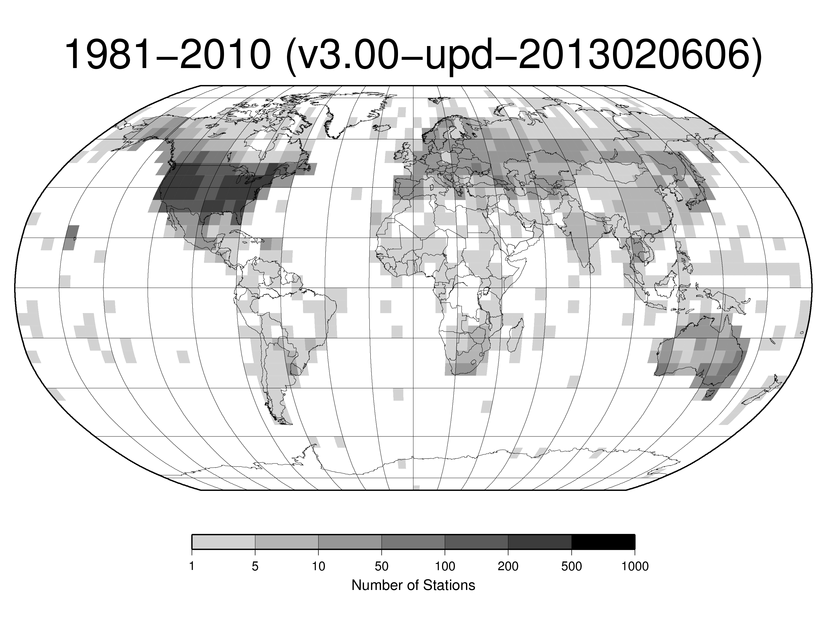
\includegraphics[trim={0cm 1.5cm 0cm 3cm}, clip, width=.425\textwidth]{bilder/Global_Historical_Climate_Network_Daily/station-counts-1981-2010-temp.png}
			\vspace{-1em}
			\caption{Wetterstationen in der Periode 1981 - 2010 die zehn Jahre lang
							 Wetterdaten übertragen haben, Quelle: Global Historical Climate Network}
		\end{figure}
	}
	\only<7|handout:0>{
	\begin{itemize}
		\item Jeder Balken repräsentiert eine Jahr aus der Periode 1850-2017
		\item Blau = kälter als der Mittelwert, Rot=Wärmer
		\item Je dunkeler die Farbe, desto extremer die Abweichung vom Mittelwert
		\item Die Trend geht klar zu höheren Temperaturen
		\item Das Logo der Scientists 4 Future
	\end{itemize}
	\begin{center}
		\url{https://s4f-dortmund.github.io/}
	\end{center}
	}

	\note<1>{
	\begin{itemize}
		\item[] Warming Stripes sind globale Zusammenfassung für ein Großteil der verfügbaren Temperaturdaten (auch S4F Logo)
		\item[] Jeder Balken Jahresmittelwert globaler Luft- und Wassertemperaturen
		\item[] Bei Interesse: Daten auf unserer Homepage verlinkt (auch für verschiedene Orte verfügbar)
	\end{itemize}
	Wie sieht die Zusammensetzung der Daten aus?
	}
	\note<2>{
	\begin{itemize}
		\item[1916] Letzte große Antarktis-Expedition (Endurance-Expedition) Leitung: Ernest Shackleton. Ziel: Den Kontinent durchqueren. Expedition scheiterte. Besonderes: alle Mitglieder unter widrigsten Umständen überlebt.
		\item[] Albert Einstein veröffentlicht die allgemeine Relativitätstheorie.
		\item[] immer mehr Wetterstationen -> genauere Messungen möglich.
	\end{itemize}
	}
	\note<3-6>{
	Immer ein 30 Jahrezeitraum hervorgehoben (später: Definition Klima)
	\begin{itemize}
		\item[vor 1891] Kaum Wetterstationen, 1-5 Stationen pro Quadrant an US-Küsten, Zentraleuropa und austalischer Ostküste
		\item[ab 1891]	Stationen die zehn Jahre lang täglich Wetterdaten übertrugen, Hier:  Temperatur (auch: Niederschlag)
		\item[] USA 50-100 Stationen pro Quadrant, Europa 1-5 Stationen, Australien 1-10 Stationen an der Küste
		\item[] Restliche Welt vereinzelt Stationen
		\item[ab 1921] Canada und Russland mit 1-5 Stationen abgedeckt
		\item[] Erste Stationen in Afrika
		\item[ab 1951] China, Indien, Argentinien, Großteile von Afrika mit 1-5 Stationen
		\item[] Australien, Europa und Teile Russlands mit 5-10 Stationen
		\item[ab 1981] Abdeckung verbessert, doch große Flächen Brasiliens, Grönlands und der Demokratischen Republik Kongo nicht abgedeck, immer noch Lücken
	\end{itemize}
	}
	\note<7>{
	Wir haben verstanden:
	\begin{itemize}
		\item[] Wie sich die globale Lufttemperatur im Laufe der Jahre verändert hat
		\item[] Wie die Lufttemperatur global gemessen wird
		\item[] Was jeder Balken in den Warming Stripes bedeutet
	\end{itemize}
	\vspace{1em}
	Gibt es Fragen?
	\vspace{1em}
	Wie wird die Zukunft aussehen?
	}
\end{frame}

\begin{frame}
	\frametitle{Warming Stripes}
	% Extrapolation der Warming Stripes
	\begin{figure}
		\centering
		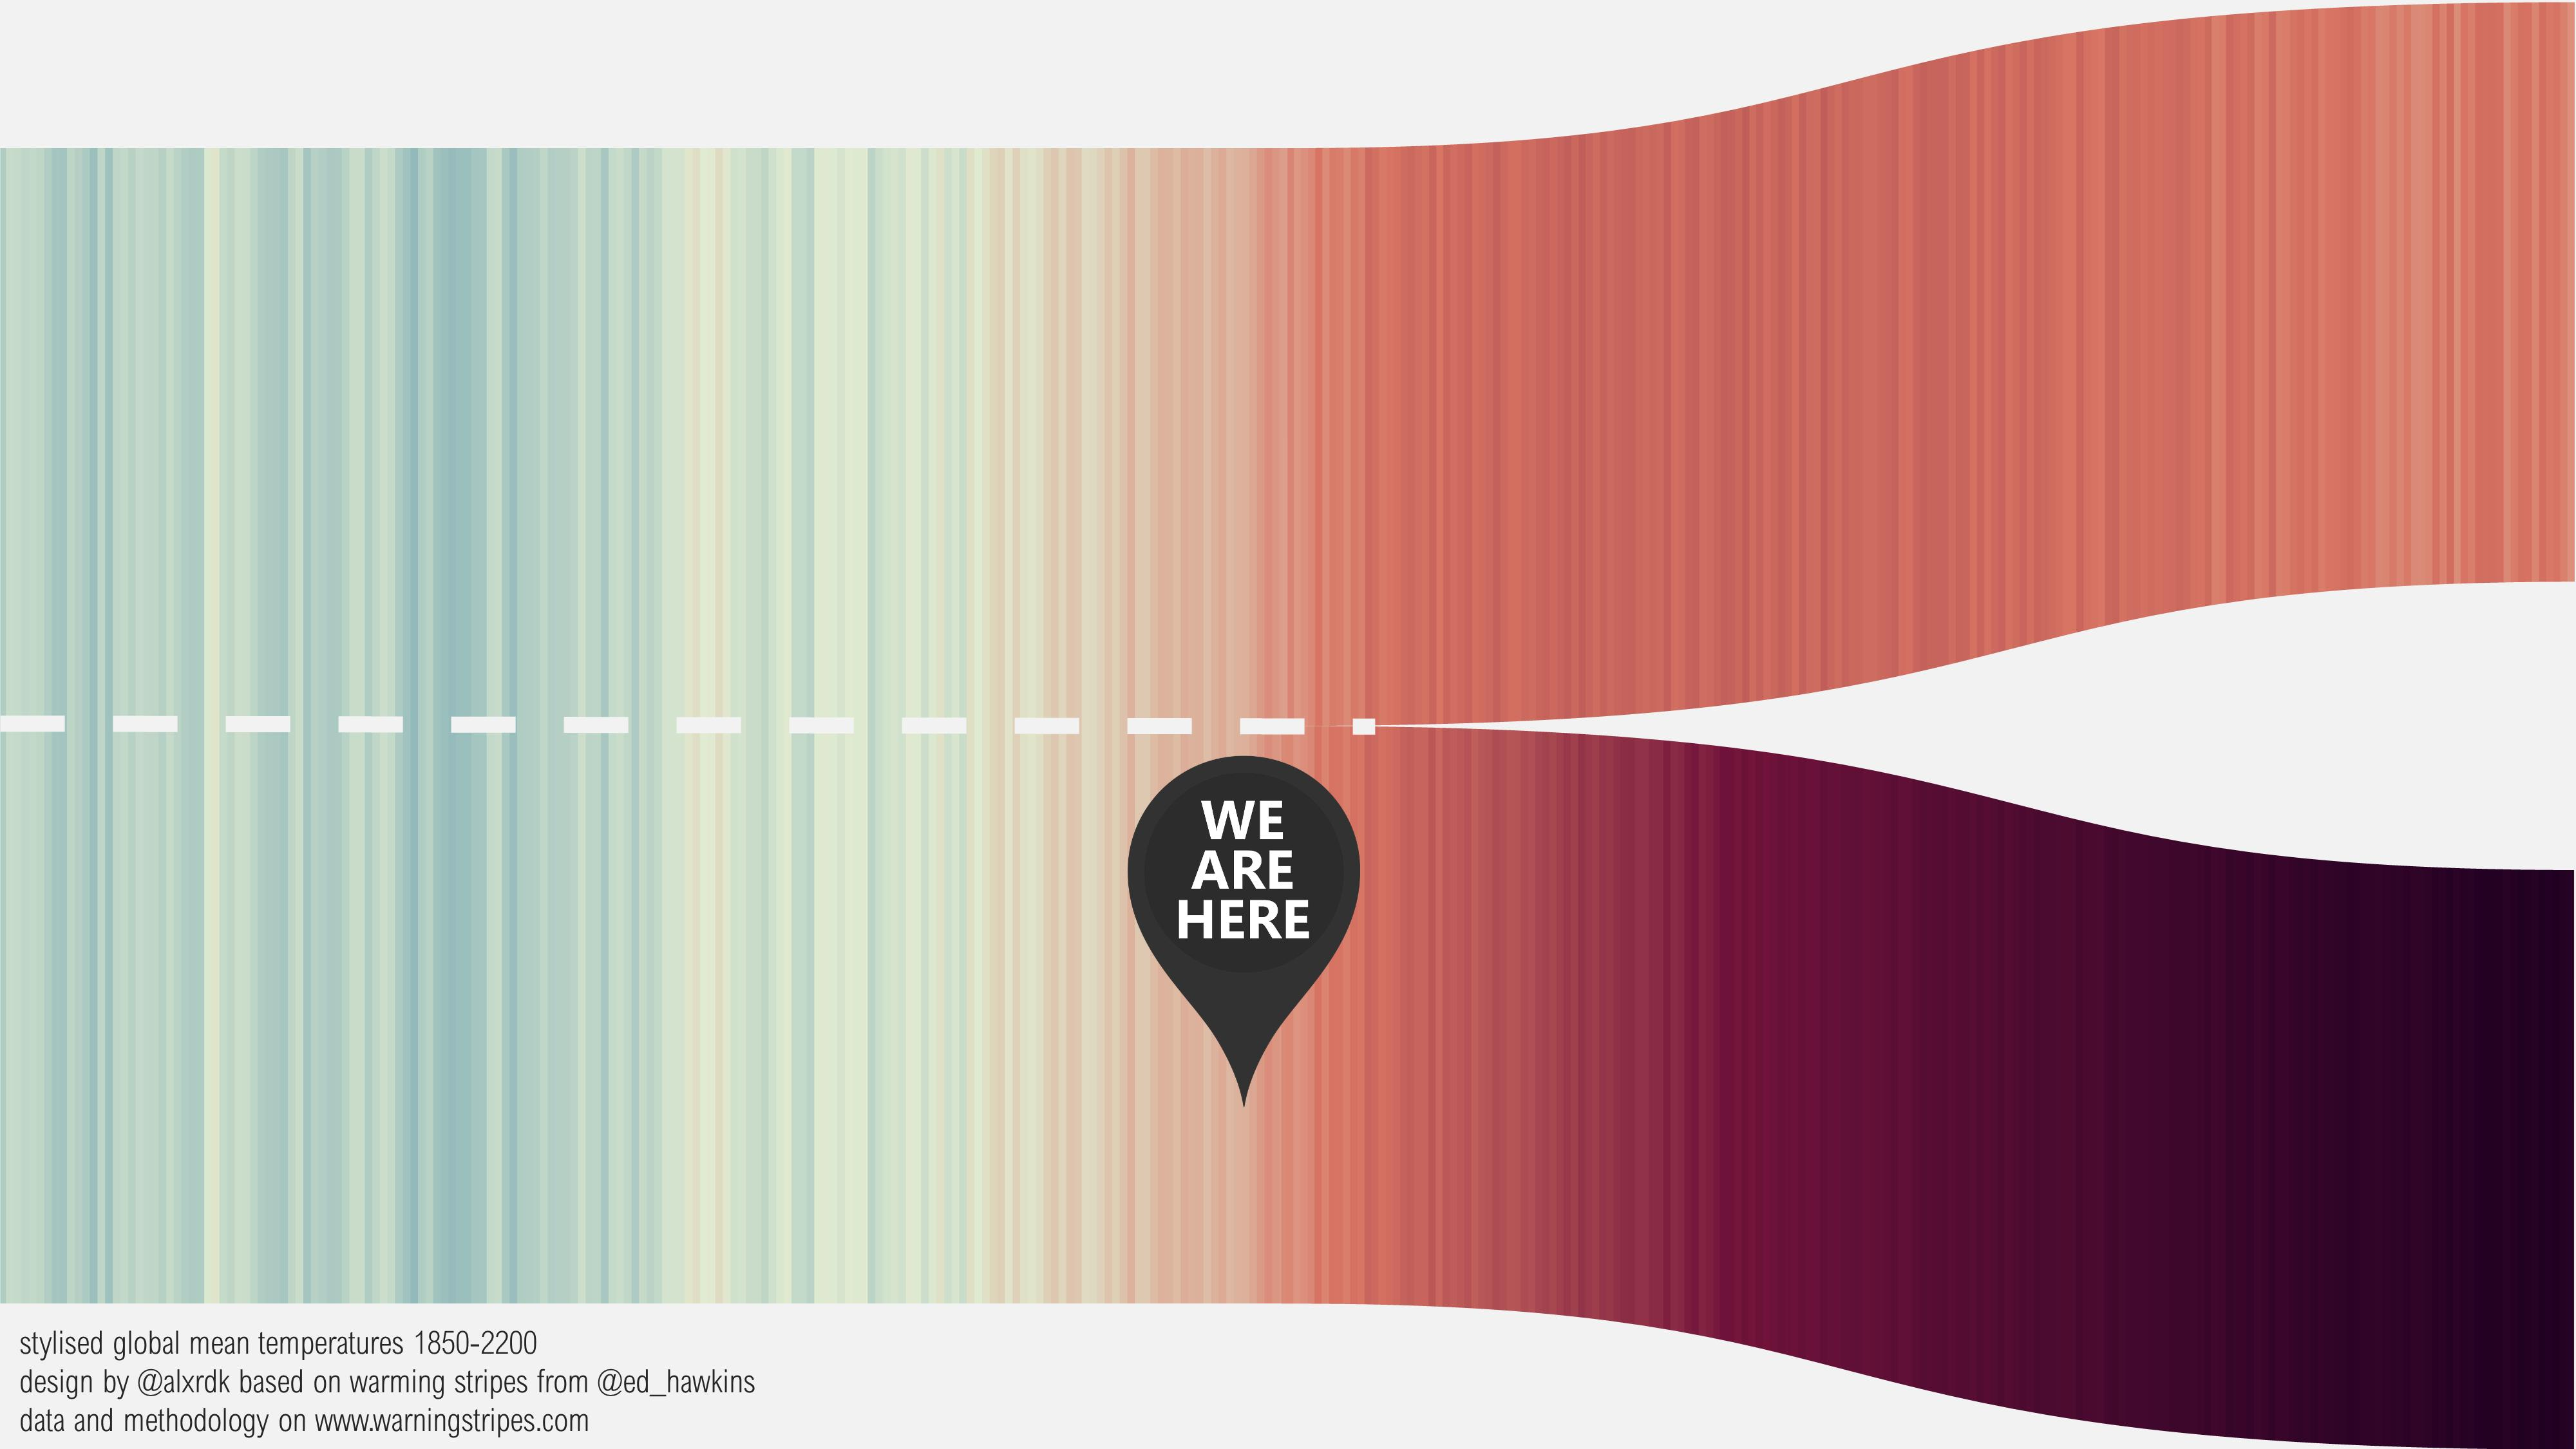
\includegraphics[width=0.55\linewidth]{bilder/warming_stripes_zukunft}
		\caption{Extrapolation der \textit{Warming Stripes} basierend auf Modellannahmen}
	\end{figure}
	\begin{itemize}
		\item In der Zukunft wird es sehr wahrscheinlich zu einer weiteren Erwärmung kommen
		\item Man kann statistische Prognosen für die Zukunft auf Basis von Modellrechnungen erstellen
		\item Der genaue Trend und die maximale Erwärmung hängen aber davon ab, was wir heute und in den nächsten Jahren tun!
	\end{itemize}

\end{frame}
